%%%%%%%%%%%%%%%%%%%%%%%%%%%%%%%%%%%%%%%%%%%%%%%%%%%%%%%%%%%%%%%%%%%%%%%%%%%
% Assessment 2: Practice exam 2019 - 2020
%%%%%%%%%%%%%%%%%%%%%%%%%%%%%%%%%%%%%%%%%%%%%%%%%%%%%%%%%%%%%%%%%%%%%%%%%%%

\begin{minipage}{0.8\textwidth}
\section{Practice exam}
\end{minipage}%
\hfill%
\begin{minipage}{0.1\textwidth}

\includegraphics[width=\linewidth]{Files/Images/pencilhand.pdf}
\end{minipage}
\vspace*{.1cm}

\underline{\textbf{Question 1 (10 points)}} \\

\begin{itemize}

\item[\textbf{1a)}] \textbf{(2 points)} Give the correct measurement levels \textit{(nominal, ordinal, interval, ratio)} for the following variables: 
\begin{itemize}
\item[$\blacksquare$] Rating (low, medium, high)
\item[$\blacksquare$] Distance (in meters)
\item[$\blacksquare$] Hair color (blonde, brown, black, red)
\item[$\blacksquare$] Temperature (in $^{\circ} C$) 
\end{itemize}
\end{itemize}

Use the following numbers to answer the next questions. \\

You are given the following sample: \\
\begin{center}
    4 \hspace{.1cm} 2 \hspace{.1cm} 5 \hspace{.1cm} 6 \hspace{.1cm} 2 \hspace{.1cm} 1 \hspace{.1cm} 2 \hspace{.1cm} 5 \hspace{.1cm} 3 \hspace{.1cm} 3 \hspace{.1cm} 7 \hspace{.1cm} 4 \hspace{.1cm} 5 \hspace{.1cm} 1 \hspace{.1cm} 7 \hspace{.1cm} 5 \hspace{.1cm} 3
\end{center}

\begin{itemize}

\item[\textbf{1b)}] \textbf{(3 points)} Calculate the mean, median, and mode of this sample.

\item[\textbf{1c)}] \textbf{(2 points)} Is the distribution of these values \textit{positively skewed} or \textit{negatively skewed}? Explain your answer using the relation between the mean, the median, and the mode.

\item[\textbf{1d)}] \textbf{(2 points)} Find the minimum, the lower quartile, the upper quartile, and the maximum of this sample. 

\item[\textbf{1e)}] \textbf{(1 point)} Give the values that are supposed to be on the dots \textit{A, B, C, D} and \textit{E} on the basis of your calculations in the previous questions. \\
\begin{center}
    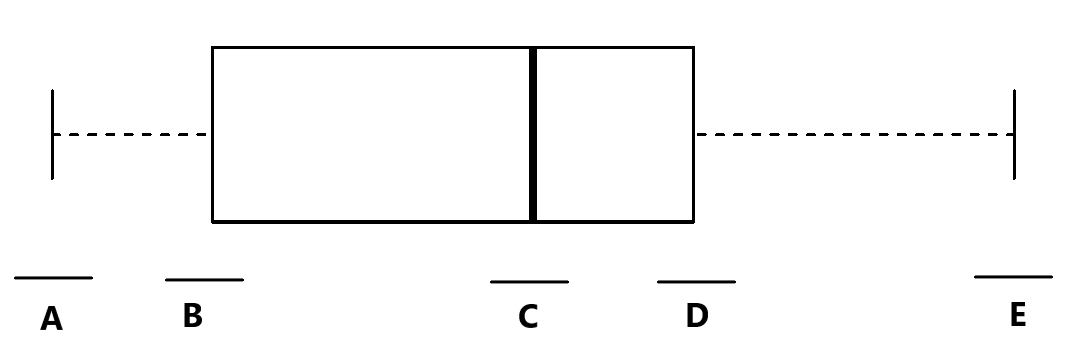
\includegraphics[width=.7\textwidth]{Files/Images/boxPlotExam.png}
\end{center}

\end{itemize}

\underline{\textbf{Question 2 (10 points)}} \\

\begin{itemize}

    \item[\textbf{2a)}] \textbf{(2 points)} Write down the Central Limit Theorem.
    
\end{itemize}
    
    One of the four assumptions for parametric tests is normally distributed data.

\begin{itemize}
    
    \item[\textbf{2b)}] \textbf{(2 points)} Explain why parametric tests require normally distributed data.
    
    \item[\textbf{2c)}] \textbf{(1 point)} What test do you use to objectively test the normality of a distribution? 
    
    \item[\textbf{2d)}] \textbf{(1 point)} What are the other three assumptions for parametric tests based on the normal distribution? 

\end{itemize}
    
    Use Table 2 on page~\pageref{table2} to answer the following two questions.
    
\begin{itemize}
    
    \item[\textbf{2e)}] \textbf{(2 points)} Calculate the 95\% upper confidence bound of the population mean $\mu$ for a random sample with sample size $n = 16$, a sample mean $\bar{x} = 38$ and a sample standard deviation $s = 4$. 
    
    \item[\textbf{2f)}] \textbf{(2 points)} Calculate the 95\% two-sided confidence interval of the population mean $\mu$ for a random sample with sample size $n = 81$, a sample mean $\bar{x} = 250$ and sample standard deviation $s = 34$.

\end{itemize}

\clearpage % Page break

\underline{\textbf{Question 3 (15 points)}} \\

Recently, there has been a lot of media attention towards the amount of lead in the water in the Netherlands. In the Netherlands, the maximum legal amount of lead per liter of water is 10 micro grams. A water researcher is hired to check the lead levels of a high school in the Netherlands. From a previous grand measurement within the school, it is known that the variance in lead in all tabs of the school is $\sigma^2 = 2.3$. The water researcher takes a sample of water from 50 tabs in the school and measures the amount of lead per liter (in micro grams) for these observations. He finds a sample mean of $\bar{x} = 7.5$.  \\

\begin{itemize}


    \item[\textbf{3a)}] \textbf{(2 points)} Write down the statistical null hypothesis $H_0$ and the statistical alternative hypothesis $H_1$ if the water researcher wants to show that, with 95\% confidence, the mean lead level (in micro grams) in the tabs is lower than the legal maximum amount.
    
    \item[\textbf{3b)}] \textbf{(2 points)} Give the critical $z$-value for this test. You may base this critical z-value on the information in Table 2 on page~\pageref{table2}.

    \item[\textbf{3c)}] \textbf{(2 points)} Calculate the $z$-value from the sample.
    
    \item[\textbf{3d)}] \textbf{(4 points)} Draw a conclusion about  on the basis of the sample z-value. Include the following four elements: 
    \begin{itemize}
        \item[$\blacksquare$] How the calculated $z$-value relates to the critical $z$-value.
        \item[$\blacksquare$] Whether this implies that $H_0$ is rejected or not.
        \item[$\blacksquare$] What this tells you about the mean lead level $\mu$ in the school.
        \item[$\blacksquare$] What type of error is relevant (\textit{type-I} or \textit{type-II}).
    \end{itemize}

\end{itemize}
    
    The figure below depicts the probability density function for a standard normal distribution. The z-score is displayed on the $x$-axis. \\
    \begin{center}
        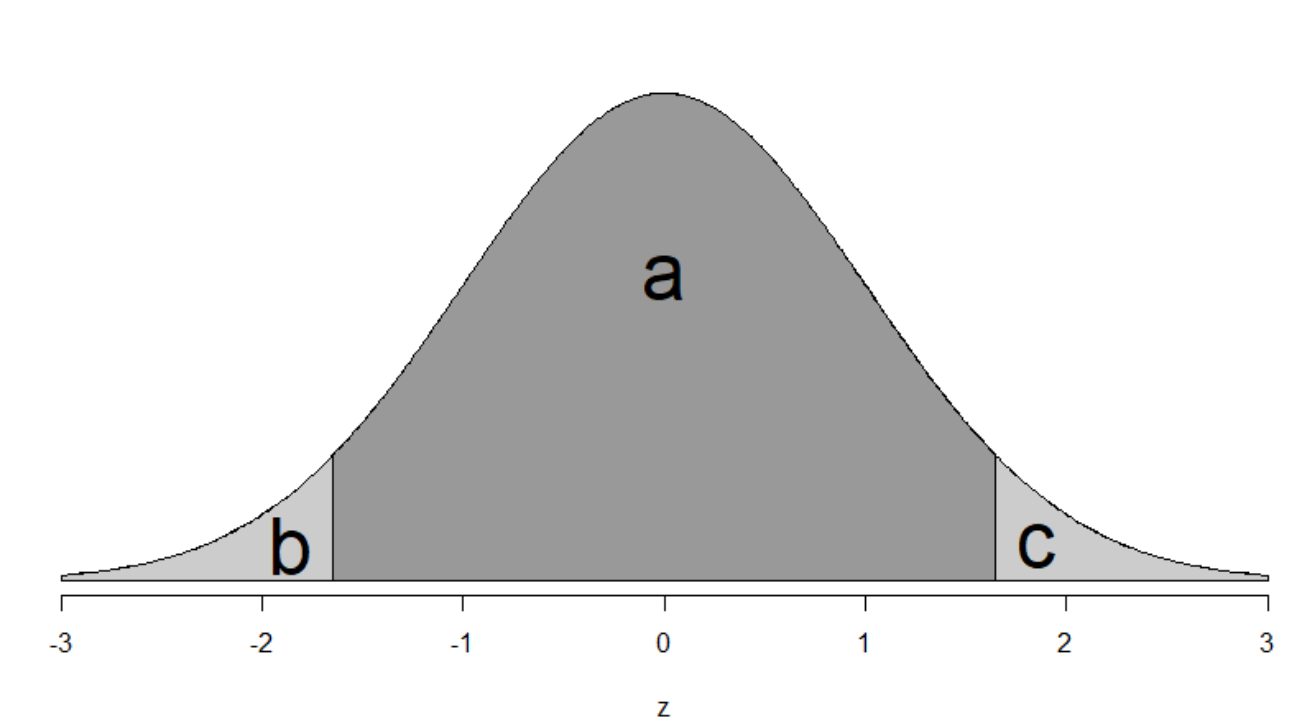
\includegraphics[width=.8\textwidth]{Files/Images/normalDistExam.png}
    \end{center}
    
\begin{itemize}

\item[\textbf{3e)}] \textbf{(3 points)} Give the letter of the area that represents the $p$-value of the last test in the figure above. Explain your answer using the definition of the $p$-value.

\item[\textbf{3f)}] \textbf{(2 points)} State whether, for this test, the $p$-value is lower or higher than 0.05. Argue how you arrived at this answer.
    
\end{itemize}

\clearpage % Page break

\underline{\textbf{Question 4 (15 points)}} \\

Researchers watched the Netflix documentary ‘The Game Changers’ and want to test the effect saturated fats have on the blood flow in a body. They did the following experiment: Ten healthy male subjects fasted for 10 hours and then got a high-fat meal. On another occasion they also fasted for 10 hours and then got a low-fat meal. Their endothelial function (how well the blood flows through small arteries to the various tissues) was measured 4 hours after this meal. \\

The mean endothelial function was 8.2\% with a standard deviation of 3.7\% after eating the high-fat meal and 13.7\% with a standard deviation of 3.3\% after the same men ate the low-fat meal. The average difference was 4.9\% with a standard deviation of the difference of 6.1\%. The researchers want to show that, with 95\% confidence, the endothelial function is significantly lower after eating a high-fat meal than after eating a low-fat meal. They have already found the critical $t$-value to be 2.262 for this case.

\begin{itemize}

    \item[\textbf{4a)}] \textbf{(11 points)} Perform a two-sample t-test for this case; include the following steps: 
    \begin{itemize}
        \item[$\blacksquare$] Explain whether this an independent or a dependent sample t-test,
        \item[$\blacksquare$] Write down the statistical hypotheses, 
        \item[$\blacksquare$] Calculate the sample $t$-score,
        \item[$\blacksquare$] Draw the conclusion; make sure you include the following four elements: 
        \begin{itemize}
            \item[$\circ$] How the calculated $t$-value relates to the critical $t$-value,
            \item[$\circ$] Whether this implies that $H_0$ is rejected or not.
            \item[$\circ$] What this tells you about the the endothelial function.
            \item[$\circ$] What type of error is relevant (\textit{type-I} or \textit{type-II}).
        \end{itemize}
    \end{itemize}
    
    \item[\textbf{4b)}] \textbf{(1 point)} When an independent two-sample t-test for the mean does not satisfy the homogeneity of variance assumption, what alternative test can you use?
    
    \item[\textbf{4c)}] \textbf{(3 points)} Explain why a dependent two-sample t-test for the mean does not have to satisfy the homogeneity of variance assumption.
    
\end{itemize}

\underline{\textbf{Question 5 (15 points)}} \\

A baby food factory has a linear regression model to predict the production price of baby food (\euro) on the basis of its sugar content (mg) and vitamins (mg) in the food. They have fitted this model to a sample ($n = 50$) of the 200 types of baby food they produce. The results indicate that, on average, the base price of baby food without any sugar or vitamins is \euro 0,60. Every mg of vitamins that the factory adds to the baby food raises its production price by \euro 0,10. Every mg of sugar that is added to the baby food raises its production price by \euro 0,15. 

\begin{itemize}

    \item[\textbf{5a)}] \textbf{(3 points)} Write down the regression equation for the linear model for all 200 types of baby food in the population. Use the names ‘price’ for the cost price (\euro) of the food, ‘sugar’ for the amount (mg) of sugar in the food, and ‘vitamins’ for the vitamins (mg) in the food. Do not fill in the values of the parameters yet. 
    
    \item[\textbf{5b)}] \textbf{(1 point)} Fill in the values of the parameters in the regression equation using the information provided by the text.

\end{itemize}

The results of the fitted model indicate that the model sum of squares is 200. The total sum of squares of the model is 250, and the residual sum of squares of the model is 50.

\begin{itemize}

    \item[\textbf{5c)}] \textbf{(1 point)} Calculate the explained variance ($R^2$) of this linear model.
    
    \item[\textbf{5d)}] \textbf{(1 point)} Interpret the $R^2$ of this linear model.
    
    \item[\textbf{5e)}] \textbf{(3 points)} Explain the problem with using the $R^2$ to compare the fit of several linear models. What alternative statistic did you learn that you can use to more reliably compare two linear models? 
    
\end{itemize}

\clearpage % Page break

In order to differentiate between baby food for 0-9, 9-12, and 12+ months, the factory’s data scientist adds two variables to the data set. The first variable (‘9-12’) contains a 1 for baby food in the category 9-12 months, and 0 otherwise. The second variable (‘12+’) contains a 1 for baby food in the category 12+ months, and 0 otherwise.

\begin{itemize}
    
    \item[\textbf{5f)}] \textbf{(1 point)} What type of variable are the variables ‘9-12’ and ‘12+’? 
    
    \item[\textbf{5g)}] \textbf{(1 point)} What test is this linear model equivalent to?
    
    \item[\textbf{5h)}] \textbf{(4 points)} Calculate the $F$-value of this linear model.
    
\end{itemize}

\underline{\textbf{Question 6 (10 points)}} \\

The Netherlands is a rainy country and historically most rain falls during the fall and early winter and is evenly spread over these four months. Students at a university in the Netherlands believe that climate change does not only affect the temperature or the amount of rainfall but also when the rain falls. They looked up the historical distribution of total rainfall in their university town for September until December on a weather website and also measured the total rainfall in the town themselves in this period in 2019. The results are shown in the table below. \\

\begin{center}
\begin{tabular}{l|c|c|c|c|c}
     & September & October & November & December & Total \\
     \hline
     Historical distribution (\%) & 23.7 & 26.3 & 25.4 & 24.6 & 100 \\
     2019 measurements (ml) & 102 & 126 & 113 & 88 & 429
\end{tabular}
\end{center} 

\begin{itemize}

    \item[\textbf{6a)}] \textbf{(8 points)} Perform a Pearson chi-square ($X^2$) test to find out if the rainfall distribution in the four months September - December in 2019 significantly deviates from the historical distribution at a 90\% confidence level. Use a critical chi-square ($df = 3$) of 6.251; include the following steps:
    \begin{enumerate}
        \item[$\blacksquare$] How the calculated $X^2$ score relates to the critical $X^2$ value.
        \item[$\blacksquare$] Whether this implies that $H_0$ is rejected or not.
        \item[$\blacksquare$] What this tells you about the 2019 rainfall distribution.
        \item[$\blacksquare$] What type of error is relevant (\textit{type-I} or \textit{type-II}).
    \end{enumerate}
    
    \item[\textbf{6b)}] \textbf{(2 points)} What is the minimum required amount for the expected frequency in all categories for the Chi-square test and what test can be done when this requirement is not met?

\end{itemize}

\underline{\textbf{Question 7 (15 points)}} \\

Your friend works as an employee of an advertising company. The company does the branding for a new startup and your friend is in charge of the advertising budget. The first six weeks of advertisement have just ended, and to assess the effectiveness of the advertising campaign your friend is interested in the relationship between the money that they have spent and the number of products that were sold as a consequence. Therefore, your friend collects data on the amount of money spent (variable $x$) and the number of products sold (variable $y$). The data is provided in the table below. \\

\begin{center}
\begin{tabular}{c|c|c}
     $i$ & $x$ & $y$ \\
     \hline
     1 & 100 & 40 \\
     2 & 120 & 60 \\
     3 & 125 & 45 \\
     4 & 110 & 30 \\ 
     5 & 170 & 70 \\
     6 & 150 & 60
\end{tabular}
\end{center} 

\clearpage % Page break

\begin{itemize}

    \item[\textbf{7a)}] \textbf{(6 points)} Calculate the covariance of the variables $x$ and $y$.
    
    \item[\textbf{7b)}] \textbf{(5 points)} Calculate the correlation between the variables $x$ and $y$.
    
\end{itemize}

Your friend wants you to assess, with 95\% confidence, whether the correlation is truly positive in the population.

\begin{itemize}
    
    \item[\textbf{7c)}] \textbf{(1 point)} Write down the statistical null hypothesis $H_0$ and the statistical alternative hypothesis $H_1$ for a left-tailed one-sided test of the correlation in the population.
    
    \item[\textbf{7d)}] \textbf{(1 point)} Calculate the sample $t$-value for a test of a correlation against zero.
    
\end{itemize}

The critical t-value for a left-tailed one-sided test with 5 degrees of freedom and 95\% confidence is 2.015.

\begin{itemize}

    \item[\textbf{7e)}] \textbf{(2 points)} Draw the conclusion about the population correlation for your friend. Include the following elements:
    \begin{itemize}
        \item[$\blacksquare$] How the calculated $t$-value relates to the critical $t$-value.
        \item[$\blacksquare$] Whether this implies that $H_0$ is rejected or not.
    \end{itemize}
    
\end{itemize}


\clearpage % Page break